% !TEX root = ../thesis.tex

\chapter{Kvantová teleportácia}

Predstavme si situáciu, že chceme na diaľku komunikovať. Chceme poslať
informáciu o stave kvantového bitu. Zaznamenať komplexné číslo úplne presne 
na číslicovom počítači nejde, a teda nemožno poslať niekomu informáciu o 
presnom stave. Takisto platí, že kvantové bity je nemožné kopírovať či
klonovať. Spôsobom akým je možné riešiť tento problém je takzvaná kvantová
teleportácia.

Medzi účastníkov komunikácie sa rozdelí dvojica previazaných bitov. Ak tieto
kvantové bity nemeriame, zachovajú si svoj stav aj previazanie nehľadiac
na fyzickú vzdialenosť medzi nimi. Teda je možné komunikovať aj na diaľku.

Uveďme si všeobecne známy príklad na kvantovú teleportáciu. Povedzme, že 
Bob chce poslať kvantový bit Alici. Najprv je nutné aby obaja vlastnili
pár previazaných kvantových bitov. Ak teraz chce Bob poslať bit Alici, jediné
čo musí spraviť je aplikovať CNOT hradlo na svoj previazaný bit, ktorý bude 
kontrolovaný kvantovým bitom, ktorý chce odoslať. Potom aplikuje Hadamardovo
hradlo na odosielaný bit a pomeria obe bity. Alici odošle informáciu o
stavoch, ktoré kolabovaním dostal. Alica z tejto informácie vie, ako má použiť
hradlá X a Z, tak aby dosiahla rovnaký stav bitu, ktorý povodne vlastnil Bob.

Týmto spôsobom je možné informáciu poslať nakoľko sa jedná o celé čísla.
Takisto nie je porušená veta o kopírovaní ani klonovaní kvantových bitov, 
nakoľko Bob svoj bit stratil.

Ukážme si to na kvantovom obvode. Vytvoríme previazaný pár kvantových bitov
ako na obrázku \ref{tel_c1}. Povedzme, že bit \(q_1\) patrí Bobovi a \(q_2\)
je Alicin.

\begin{figure}[H]
	\centering 
	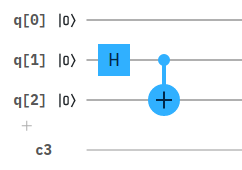
\includegraphics[width=.5\textwidth]{figures/tel_c1.png} 
	\caption{Previazanie kvantových bitov na kvantovú teleportáciu.}
    \label{tel_c1}
\end{figure}

Ako bolo spomenuté, na to aby mohol Bob poslať bit \(q_0\), musí aplikovať
CNOT a následne Hadamardovo hradlo, tak ako na obrázku \ref{tel_c2}.

\begin{figure}[H]
	\centering 
	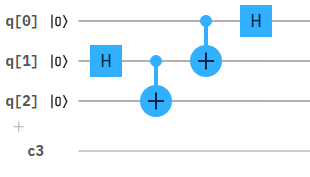
\includegraphics[width=.5\textwidth]{figures/tel_c2.png} 
	\caption{Obvod popisujúci kvantovú teleportáciu.}
    \label{tel_c2}
\end{figure}

Bob pomeria svoje bity a pošle tieto merania Alici. Alica na základe týchto
meraní vie, že ak
\begin{itemize}
    \item[] Bobov bit \(q_0\) nadobudne stav \(1\), aplikuj hradlo \(Z\) na 
            \(q_2\)
    \item[] Bobov bit \(q_1\) nadobudne stav \(1\), aplikuj hradlo \(X\) na 
            \(q_2\)
\end{itemize}

\subsection*{IBM Quantum Experience výsledky}
Dokončime obvod. Povedzme, že posielame stav \(\ket{1}\), preto pridáme 
hradlo \(X\) na začiatok obvodu a plikujeme na \(q_0\). Na koniec pridáme 
podmienené aplikácie hradiel \(Z\) a \(X\). IBM QX podporuje variantu hradla
\(CNOT\), kde namiesto preklopenia \(X\) aplikujeme \(Z\). Výsledný obvod aj
s meraniami je na obrázku \ref{tel_qx_results}.

\begin{figure}
	\centering 
	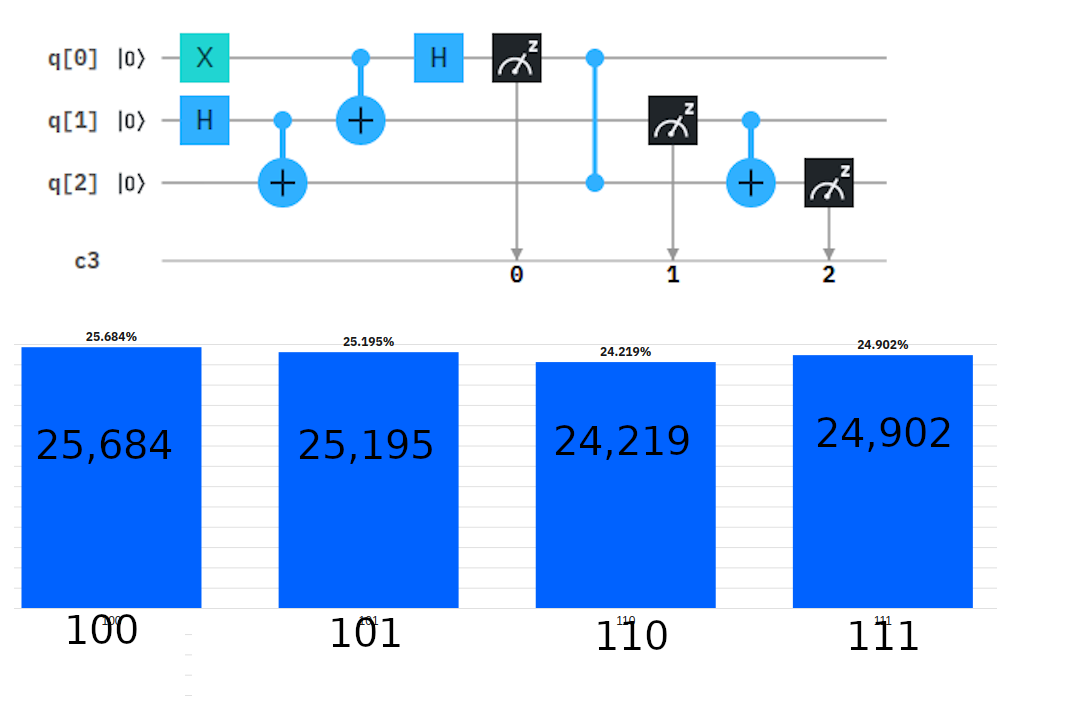
\includegraphics[width=.7\textwidth]{figures/tel_qx_results.png} 
	\caption{Výsledky príkladku kvanovej teleportácie.}
    \label{tel_qx_results}
\end{figure}

Podľa výslekov je jasné, že teleportácia bola úspešná. Najhlavnejší bit 
všetkých výsledkov je \(1\). To znamená, že Alicin kvantový bit vždy nadobudne
taký stav aký mal pôvodne Bob, čo bolo \(\ket{1}\).

\subsection*{Pravdepodobnostný model}
Definujeme kvantový obvod pre program v jazyku Haskell.

\begin{code}
let l1 = Level [E, H, E] True
    l2 = Level [E, Cc, Ct] True
    l3 = Level [Cc, Ct, E] True
    l4 = Level [H, E, E] True
    c = [l1, l2, l3, l4]
    st = StateTree 1 [q1, q0, q0] []
    rt = RT st []
\end{code}
   
Bit \(q_0\) nastavýme na stav \(\ket{1}\), ostatné na \(\ket{0}\). V našom
pravdepodobnostnom modeli nejestvuje možnosť podmienených aplikácií hradiel,
tak si budeme musieť vystačiť s neúplnou teleportáciou.

Fiktívne meranie je nastavené za každým levelom, výsledky meraní su v tabuľke
\ref{tel_results}.

\begin{table}
\centering

\begin{tabular}{|c|c|}
\hline
0.50 & 0.49 \\ 
100 & 110 \\ 
\hline
\end{tabular}

\begin{tabular}{|c|c|c|c|}
\hline
0.25 & 0.249 & 0.25 & 0.25 \\ 
101 & 111 & 100 & 110 \\ 
\hline
\end{tabular}

\begin{tabular}{|c|c|c|c|c|c|c|c|}
\hline
0.25 & 0.249 & 0.0 & 0.0 & 0.25 & 0.25 & 0.0 & 0.0 \\ 
101 & 111 & 101 & 111 & 100 & 110 & 100 & 110 \\ 
\hline
\end{tabular}

\begin{tabular}{|c|c|c|c|c|c|c|c|}
\hline
0.125 & 0.1249 & 0.1249 & 0.1249 & 0.125 & 0.125 & 0.125 & 0.1249 \\ 
001 & 011 & 101 & 111 & 000 & 010 & 100 & 110 \\ 
\hline
\end{tabular}

\caption{\label{tel_results} Výsledky merania experimentu kvantovej
teleportácie pomocou
pravdepodobnostného modelu. Ohraničené riadky vymedzujú výsledky v jednotlivých
 časoch merania. Každá bunka obsahuje pravdepodobnosť dosiahnutia stavu a 
daný stav systému.}
\end{table}

Opäť pripomeňme, že poradie bitov vo výsledkoch z pravdepodobnostného modelu
a výsledkoch IBM QX je opačné. Pozornému oku neunikne, že v niektorých 
prípadoch výsledky po použití hradiel \(X\) a \(Z\) nebudú dávať správny 
výsledok. Je nutné podotknúť, že pravdepodobnostný model nepracuje až tak 
na základe vstupných stavov kvantových bitov v obvode ako na základe
matematikého modelu pravdepodobností dosiahnutia stavov \(\ket{0}\) a 
\(\ket{1}\). Takisto je vydno, že niektoré možnosti sú nedosiahnuteľné.
Teda výsledky pravdepodobnostného modelu sú narozdiel od IBM QX odvodzované od
všeobecných stavov kvantových bitov \(\ket{\psi}\) a vstupné hodnoty stavov
týchto bitov sú použité len na upravednie pravdepodobností do finálnej podoby.
